\documentclass[12pt, letterpaper]{article}
\usepackage{graphicx} % Required for inserting images
\usepackage{hyperref}
\usepackage{listings}
\usepackage{amssymb}
\usepackage{amsmath}
\usepackage[english]{babel}
\usepackage{nicefrac, xfrac}
\usepackage{mathtools}
\usepackage[table,xcdraw]{xcolor}
\definecolor{light-gray}{gray}{0.95}
\definecolor{sap}{RGB}{130, 36, 51}
\definecolor{lg}{RGB}{102, 161, 95}
\usepackage[paper=a4paper,left=20mm,right=20mm,bottom=25mm,top=25mm]{geometry}
\newcommand{\code}[1]{\colorbox{light-gray}{\texttt{#1}}}
\newcommand{\codee}[1]{\colorbox{white}{\texttt{#1}}}
\newcommand{\acc}{\\\hphantom{}\\}
\newcommand{\dete}{{\rightarrow}}
\newcommand{\fdot}{{\(\bullet\) }}
\newcommand{\comm}[1]{\color{lg}\textit{\hphantom{spaz}// \text{#1}}\color{black}}
\newcommand{\boxedMath}[1]{\begin{tabular}{|c|}\hline \texttt{#1} \\ \hline\end{tabular} :}
\title{Basi di Dati 2}
\author{Marco Casu}
\date{\vspace{-5ex}}
\begin{document}



\maketitle
\begin{figure}[h]
    \centering{
    
\includegraphics[width=1\textwidth ]{images/copertina.jpeg}
    }
\end{figure}
\newpage 
\tableofcontents
\newpage
\section{Introduzione}
Questo corso non è ristretto esclusivamente alla progettazione di basi di dati, bensì fornisce 
cenni sulla progettazione di software di grandi dimensioni, supportati da basi di dati reali.\acc 
Un cliente (committente) fornisce delle specifiche riguardo un progetto che bisogna sviluppare, 
esso stesso non sa come verrà implementato o quali sono nello specifico tutte le funzionalità, 
un insieme di ingegneri del software, progettisti, e programmatori si occuperanno di "tirare su" il 
lavoro completo nel tempo, e varie figure professionali verranno necessariamente coinvolte.\acc 
\textit{Tempi per un progetto software complesso} :\begin{itemize}
    \item Capire il problema e cosa vuole realmente il cliente : \(33\%\) del tempo totale.
    \item Progettazione, capire come implementare le richieste del cliente : \(50\%\) del tempo totale.
    \item Effettiva realizzazione (sviluppo del codice) : \(17\%\) del tempo totale.
    \item Del tempo extra per i test di verifica e la manutenzione.
\end{itemize}
\subsection{Contesto Organizzativo}
Le figure professionali \textit{chiave} coinvolte nel progetto sono dette \textbf{attori}, generalmente
sono :\begin{itemize}
    \item Committente ed Esperti del dominio 
    \item Analisti e Progettisti
    \item Programmatori 
    \item Utenti finali e Manutentori
\end{itemize}
Qual'è la differenza tra analisti e progettisti? E di cosa si occupano gli esperti del dominio?\acc 
Il \textbf{dominio} dell'applicazione è l'insieme di informazioni necessarie da conoscere per poter lavorare 
ad un progetto che fa riferimento ad uno specifico ambito, ad \textit{esempio}, un applicazione che si occupa 
di registrare e gestire le contravvenzioni stradali, vedrà sicuramente nel suo dominio il codice stradale 
e le informazioni legislative. \acc L'esperto del dominio è una figura, appunta esperta, del dominio inerente 
al progetto in questione, viene pagata dal committente e funge da consulente durante lo sviluppo.
\subsection{Ciclo di Vita del Software}
È possibile suddividere lo sviluppo di un software in macro-fasi principali.\begin{enumerate}
    \item \textbf{Studio di fattibilità} - Ci si approccia al progetto valutando i costi per realizzarlo ed 
    i benefici, si pianificano le attività e le risorse del progetto, umane ed economiche, e si individua l'ambiente
    di programmazione hardware e software. 
    \item \textbf{Raccolta dei requisiti} - Bisogna capire \textit{cosa il sistema deve fare}, scrivere in prosa 
    una documentazione che descriva precisamente le usabilità del progetto, sintetizzando i requisiti, che spesso 
    sono contraddittori, trovando i giusti compromessi.
    \item \textbf{Analisi concettuale dei requisiti} - Sono coinvolti gli analisti, che produrranno uno schema 
    matematico del progetto, dettagliato per filo e per segno, che definirò cosa l'applicazione deve fare 
    indipendentemente dal come. Lo schema prima citato è detto \textit{schema concettuale}, e sarà la base 
    da cui partire per la progettazione.
    \item \textbf{Progettazione (design) dell'applicazione} -  Bisogna capire \textit{come} il sistema 
    realizzerà le sue funzioni, entra in gioco il progettista, che definirà l'architettura volta ad ospitare 
    il software e l'insieme delle tecnologie necessarie.
    \item \textbf{Realizzazione} - Una volta che si hanno le linee guida per la realizzazione, composte 
    nelle fasi precedenti, si delega la scrittura del codice ai programmatori, che non sono coinvolti nel resto 
    e non devono necessariamente essere a conoscenza di cosa stanno facendo, ma esclusivamente produrre 
    le funzioni richieste.
    \item \textbf{Verifica, esercizio e manutenzione} - Le diverse componenti dell'applicazione vengono 
    integrate. Una volta che il progetto è realizzato e pronto alla 
    messa in esercizio, si passa da una fase di testing ad una fase di utilizzo effettivo, l'applicazione verrà 
    monitorata durante l'esercizio ed eventuali correzzione verranno prodotte.
\end{enumerate}
Si osservi il seguente diagramma rappresentante il \textbf{modello a spirale} di realizzazione : \begin{center}
    \includegraphics[width=0.65\textwidth ]{images/cicloDiVita.eps}
\end{center}
Tutto il progetto viene costruito in maniera "iterativa", si dice che lo sviluppo del software sia 
\textit{agile}, si comincia raccogliendo i requisiti strettamente necessari, per poi procedere all'analisi 
considerando tali requisiti, con l'andare avanti delle fasi portando alla realizzazione di una prima versione 
del software, pronta ad essere messa in esercizio, implementante esclusivamente le funzionalità di base, tale 
versione renderà chiare le idee al committente che potrà fornire nuovi requisiti, in modo tale da ricominciare il ciclo.\acc 
Nulla vieta alle varie fasi di essere eseguite in parallelo, ad esempio, nel tempo \(t_0\) vengono stilati 
i requisiti per la prima versione del software, nel tempo \(t_1\) gli analisti iniziano a produrre il modello della versione 1, ma 
possono essere nel mentre stilati i requisiti della versione 2, al tempo \(t_3\), com'è di facile intuzione : 
 Si raccolgono i requisiti per la versione 3, si produce il modello della versione 2, si progetta la versione 1.
 \section{Il linguaggio UML}
Il linguaggio UML, acronimo di \textit{Unified Modeling Language}, nasce con l'intento di definire un 
linguaggio logico-matematico e formale per la progettazione del software. Utilizza dei diagrammi con lo scopo di 
"sintetizzare" un linguaggio puramente logico. \acc 
Verrà utilizzato l'UML per modellare il dominio applicativo ed i dati di interesse, utilizzeremo il cosiddetto 
\textbf{diagramma delle classi e degli oggetti}. Un \textit{oggetto} modella un elemento del dominio di business, 
la cui esistenza è "autonoma", e può essere identificato appunto come un "oggetto" del mondo reale, identifica una classe, 
di cui è "estensione", in maniera similare ai linguaggi object-oriented\acc Sarà importante concentrarsi sulle classi 
piuttosto che sugli oggetti specifici, una classe definisce un nome identificativo, degli attributi e delle 
operazioni.\begin{center}
    \includegraphics[width=\textwidth ]{images/umlBase.eps}
\end{center}
Una classe permette di modellare oggetti dello specifico tipo definito da essa, un oggetto ha un identificatore 
univoco (sottolineato), possono però esistere due oggetti identici, a patto che differiscano per 
l'identificatore.
\subsection{Associazioni e Link}
Un \textit{associazione} definisce un legame fra due oggetti istanza di due classi diverse, si denota con una freccia o linea che collega due classi, 
e deve presentare un titolo, ad esempio, un oggetto di tipo \textit{Libro}, può essere associato ad un oggetto 
di tipo \textit{Persona} tramite un'ipotetica associazione \textit{autore}.\begin{center}
    \includegraphics[width=\textwidth ]{images/associazione.eps}
\end{center}
Un \textit{link} non è altro che il corrispettivo delle associazioni, ma sugli oggetti istanza delle classi. Due oggetti 
identici possono esistere, ma due link identici fra due oggetti no, si immagini l'esempio precedente di autore, 
non avrebbe senso che una persona sia due volte autore dello stesso libro.\begin{center}
    \includegraphics[width=0.8\textwidth ]{images/2link.eps}
\end{center}
\subsubsection{Classi Ponte e Molteplicità}
Si consideri adesso il seguente esempio, si vuole progettare un'applicazione che gestire le prenotazioni di un 
hotel, e si produce il seguente modello UML, con le classi \textit{Hotel} e \textit{Persona} unite dall'associazione 
"prenota", cosa succederebbe se una persona volesse prenotare 2 volte lo stesso hotel? \begin{center}
    \includegraphics[width=0.7\textwidth ]{images/hotelSbagliato.eps}
\end{center}
Non è giusto modellare la prenotazione come un associazione, in quanto vogliamo che le prenotazioni esistano come 
oggetti autonomi, e che uno stesso cliente possa prenotare più volte lo stesso hotel, si necessita di una classe 
prenotazione che si occupi di tale relazione, una classe di questo tipo è detta \textbf{classe ponte}, e nel 
caso degli hotel, viene 
implementata nel seguente modo : \begin{center}
    \includegraphics[width=0.9\textwidth ]{images/hotelGiusto.eps}
\end{center}
Ovviamente, fra le stesse due classi, possono esistere più associazioni diverse, ad esempio, le classi 
\textit{Libro} e \textit{Persona}, potrebbero essere relazionate da \textit{autore} ed \textit{editore}. Inoltre, 
un oggetto di una classe \(C_1\), può essere collegato tramite link a due oggetti diversi di una stessa classe 
\(C_2\), ciò è valido, ma potrebbe causare alcuni errori logici : \begin{center}
    \includegraphics[width=1\textwidth ]{images/multError.eps}
\end{center}
Nonostante lo schema relazionale permetta tali istanze, il fatto che una persona sia nata in due città differenti 
non rispetta i vincoli del mondo reale, il diagramma è quindi troppo \textit{lasco}, appositamente per situazioni 
di questo tipo, esistono dei costrutti, detti \textbf{vincoli di molteplicità} sulle associazioni, che restringono 
il possibile numero delle istanze, imponendo delle restrizioni sul numero di link che possono esistere fra due classi.
\begin{center}
    \includegraphics[width=1\textwidth ]{images/molteplicita.eps}
\end{center} 
I vincoli di molteplicità vengono aggiunti ai terminali della linea associazione : \begin{itemize}
    \item il vincolo \textbf{0..*} posto al terminale della classe \textit{A}, in associazione con la 
    classe \textit{B} implica che ogni istanza della classe \textit{A}, dovrà essere coinvolta in un numero di link 
    dell'associazione in questione, che va da 0 ad un qualsiasi numero (ogni istanza di \textit{A} può essere legata 
    ad un numero qualunque di istanze di \textit{B}).
    \item il vincolo \textbf{1..1} posto al terminale della classe \textit{A}, in associazione con la 
    classe \textit{B} implica che ogni istanza della classe \textit{A}, dovrà essere coinvolta in un numero di link 
    dell'associazione in questione, che va da 1 ad 1 (ogni istanza di \textit{A} sarà collegata ad una sola 
    istanza di \textit{B}).
    \item (caso generale) il vincolo \textbf{\(k\)..\(n\)} posto al terminale della classe \textit{A}, in associazione con la 
    classe \textit{B} implica che ogni istanza della classe \textit{A}, dovrà essere coinvolta in un numero di link 
    dell'associazione in questione, che va da \(k\) ad \(n\).
\end{itemize}\begin{center}
    \includegraphics[width=\textwidth ]{images/esempioAuto.eps}
\end{center}
Si considerino i seguenti requisiti : Si vogliono rappresentare i sovrani 
di un regno, di ognuno di loro, è importante considerare il predecessore 
ed il successore, è possibile in UML creare un link fra due oggetti della 
stessa classe, con un associazione sulla stessa classe : \begin{center}
    \includegraphics[width=0.5\textwidth ]{images/sovrani.eps}
\end{center}
Risulta però \textit{obbligatorio} dare dei nominativi ai \textbf{ruoli}
posti ai terminali dell'associazione, altrimenti sarebbe impossibile quale 
delle due classi sta interpretando il ruolo di successore o predecessore. 
Vorremmo inoltre che ogni sovrano, eccetto il primo e l'ultimo, abbia esattamente 
un successore ed un predecessore, ma il diagramma in questione permette a qualunque 
sovrano di violare tali vincoli del mondo reale.
\subsubsection{Associazioni con Attributi}
Si vuole progettare un sistema che gestisca gli esiti (voti in 30esimi) di 
più esami sostenuti dagli studenti di un corso di laurea, esisteranno sicuramente 
le classi \textit{Studente} ed \textit{Esame}.\acc 
Il problema, è che non è possibile utilizzare una classe ponte, in quanto 
deve essere impossibile per uno studente, superare lo stesso esame più di una volta. Sarebbe 
naturale inserire il voto dell'esame in questa ipotetica classe ponte, ma sapendo che non 
è utilizzabile, dove verrà inserito l'attributo \textit{voto}?
\begin{center}
\includegraphics[width=0.8\textwidth ]{images/votoSbagliato.eps}
\end{center}
 Chiaramente, non posso inserirlo nella classe \textit{Studente}, in quanto 
 ogni studente avrebbe un unico voto per ogni esame, e non posso inserirlo 
 nella classe \textit{Esame}, dato che tutti gli studenti avrebbero lo 
 stesso voto nello stesso esame. \acc 
 È possibile considerare degli \textbf{attributi di associazione}, dando 
 ad ogni link di \textit{testSuperato}, il corrispettivo valore del voto, risulta 
 una soluzione naturale, in quanto il voto è assegnato ad ogni superamento di un test :\begin{center}
    \includegraphics[width=0.8\textwidth ]{images/votoGiusto.eps}
    \end{center} 
Anche se simile, il riquadro \textit{votoSuperato} non rappresenta una 
classe, in UML è detta \textit{association class}, e anche essa può essere collegata ad 
altre classi, si supponga ad esempio che vogliamo associare ad ogni 
test superato, anche il docente che ha verbalizzato il voto, basta 
collegare l'associazione con attributi ad una classe \textit{Docente} : \begin{center}
    \includegraphics[width=0.8\textwidth ]{images/conDocente.eps}
    \end{center} 
\subsection{Tipi di Dato} \label{dataType}
Per ogni attributo di ogni classe abbiamo visto essere necessario 
considerare il tipo del dato, esiste infatti un insieme di tipi di 
dato \textit{concettuali}, che siano facilmente implementabili 
in modo ovvio su qualsiasi sistema o linguaggio di programmazione.\begin{center}
    \code{Intero, Reale, Booleano, Data, Ora, DataOra}
\end{center} Il fatto è che il linguaggio UML vuole modellare situazioni 
reali, è quindi necessario considerare dei tipi di dato più restrittivi ed 
accurati, nell'esempio precedente degli esami, che tipo di dato dovrebbe 
assumere l'attributo \textit{voto}? \acc Non possiamo dargli il tipo "intero", 
in quanto ciò permetterebbe ad un voto di assumere anche valori come -5 o 25013, e 
non avrebbe alcun senso per essere un voto di un esame. È possibile considerare 
dei \textbf{vincoli} con un criterio di \textit{specializzazione}, allo scopo di 
restringere l'insieme dei possibili valori che può assumere un determinato 
attributo, ad esempio : \begin{center}
    \includegraphics[width=0.7\textwidth ]{images/tipiDato.eps}
    \end{center} 
In UML, il tipo \(k..n\), indica un \textit{intervallo di numeri interi}, 
l'attributo in questione può assumere valori da un minimo di \(k\) ad un 
massimo di \(n\), nel caso del voto, assume valori da 18 a 30.\acc 
È possibile anche definire esplicitamente l'insieme di valori che possono essere 
assunti, tramite il tipo \textit{enumerativo} :
\begin{center}
    \includegraphics[width=\textwidth ]{images/enum.eps}
\end{center} 
Se volessimo rappresentare un indirizzo? Si possono creare dei tipi di 
dato \textbf{composti}, costituiti da più tipi di dato, con le eventuali 
restrizioni (è possibile definire i tipi di dato in un documento separato) : 
\begin{center}
    \includegraphics[width=\textwidth ]{images/datiComposti.eps}
\end{center} 
Possono essere definiti anche dei \textit{vincoli di molteplicità} sugli 
attributi, permettendo ad un oggetto di avere più campi di uno stesso attributo, ad 
esempio, una classe \textit{Utente} di un social network, può permettere ad ogni utente di 
avere più indirizzi email, allora l'attributo si definirà nel seguente modo : \begin{center}
    email : String [1..*]\comm{uno o più indirizzi email}
\end{center}
\subsection{Vincoli}
Il linguaggio UML permette di aggiungere i cosiddetti \textbf{vincoli d'integrità}, delle asserzioni che hanno lo 
scopo di restringere il possibile insieme delle istanze, ossia degli oggetti ammessi. Una tipologia di vincolo è 
quella dell'\textit{identificazione di classe}, è un vincolo che, impone a due differenti istanze di una classe, 
di non poter avere uno o più attributi coincidenti.\acc 
Un tipico esempio può essere fatto per una classe \code{Persona}, che presenta un attributo \code{codice fiscale},
è necessario un vincolo di identificazione di classe, che imponga a due differenti istanze di \code{Persona} di non 
avere lo stesso \code{codice fiscale}. \acc Tale vincolo può essere aggiunto anche su un insieme di attributi, 
se il vincolo è su \code{x} ed \code{y}, due oggetti istanza possono coincidere su \code{x} ma non su \code{y}, oppure 
su \code{y} ma non su \code{x}, non possono essere coincidenti su entrambi.\begin{center}
    \includegraphics[width=\textwidth ]{images/identificazione.eps}
\end{center} 
Affianco all'attributo in questione, si inserisce la dicitura \code{\{id\}}, possono coesistere anche identificazioni 
di classe differenti, di solito si usano le diciture \code{\{id1\}, \{id2\}...,\{id$k$\}} ecc.\acc Un vincolo di 
identificazione può anche coinvolgere un'associazione. Se il vincolo è posto su un'associazione da 
\code{x} ad \code{y}, e su un attributo
della classe \code{x}, 
vuol dire che non possono esistere due istanze di \code{x} con l'attributo in questione coincidente, che hanno un 
link verso la medesima istanza di \code{y} :\begin{center}
    \includegraphics[width=\textwidth ]{images/vincoloAss.eps}
\end{center} 
Attenzione : Un vincolo di identificazione di classe può coinvolgere esclusivamente attributi a molteplicità 
$1..1$ e associazioni in cui il ruolo della classe ha molteplicità $1..1$.
\subsection{Generalizzazione delle Classi}
Risultano molto comuni, situazioni in cui diverse classi condividono gli stessi attributi. Il concetto di classe e sotto-classe 
è ben noto, già dal corso di
\color{blue}\href{https://github.com/CasuFrost/University_notes/blob/main/Primo%20Anno/Secondo%20Semestre/Metodologie%20di%20Programmazione/Appunti%20Metodologie%20di%20programmazione.pdf}{
    Metodologie di Programmazione
}\color{black}, dove si è affrontata la programmazione orientata agli oggetti, in UML, è possibile definire delle relazioni 
di classe e sotto-classe, che però risultano ben più "potenti" e flessibili del corrispettivo in Java.\begin{center}
    \includegraphics[width=\textwidth ]{images/sottoclasse..eps}
\end{center} 
Tutti gli attributi, associazioni e le molteplicità della superclasse sono ereditati dalla sottoclasse. Ovviamente 
la relazione di classe-sottoclasse può essere re-iterata, costruende un "albero" gerarchico, in cui ogni 
livello eredita gli attributi ed associazioni del livello superiore.\acc La classe \code{Studente} sarà sottoclasse di 
una classe \code{Persona}, se quest'ultima è in una associazione \code{nascita} con una classe \code{Città}, anche 
\code{Studente} lo sarà, una sottoclasse di \code{Studente}, ad esempio, \code{StudenteStraniero}, erediterà sia 
le proprietà di \code{Studente} che quelle di \code{Persona}. \begin{center}
    \includegraphics[width=0.6\textwidth ]{images/studStraniero.eps}
\end{center} 
Tutto ciò, aumenta significativamente la complessità dello schema relazionale e del livello degli oggetti, nulla vieta 
ad un oggetto di appartenere a più classi, nell'esempio precedente, un istanza di \code{StudenteStraniero}, è anche 
istanza di \code{Studente} e \code{Persona}, però la classe più \textit{specifica} alla quale fa riferimento è appunto 
\code{StudenteStraniero}, si definisce per un oggetto quindi l'insieme delle sue classi più specifiche.
\begin{center}
    \includegraphics[width=0.8\textwidth ]{images/ClassiSpec.eps}
\end{center} 
Se diverse classi sono sottoclassi di una classe comune, è possibile utilizzare il costrutto "\textit{is-a}" per 
denotare tale comportamento del modello. Si ha una classe \code{a}, e due classi \code{b} e \code{c}, entrambe 
sottoclassi di \code{a} tramite il costrutto "\textit{is-a}", un oggetto istanza di \code{a} potrà essere anche :\begin{itemize}
    \item Sia istanza di \code{b} che di \code{c}.
    \item Solo istanza di \code{b}.
    \item Solo istanza di \code{c}.
    \item Ne istanza di \code{b}, ne di \code{c}.
\end{itemize}\begin{center}
    \includegraphics[width=0.7\textwidth ]{images/isa.eps}
\end{center} 
In questo caso \code{Studente} e \code{Lavoratore} fanno parte della \textbf{stessa generalizzazione}, ossia \code{occupazione},
nulla vieta ad una classe di essere superclasse di generalizzazioni distinte : \begin{center}
    \includegraphics[width=0.7\textwidth ]{images/isa2.eps}
\end{center} 
In questo modello, una Persona può essere : Uomo, Donna, Uomo e Donna, ne Uomo ne Donna, e contemporaneamente 
può essere Studente, Lavoratore, Studente e Lavoratore o nessuno dei due. Risulta ambiguo il fatto che una persona 
possa essere sia uomo che donna, è necessario imporre allo schema, che ogni persona sia o Uomo o Donna, è possibile 
considerare dei \textbf{criteri sulle generalizzazioni}, che si occupano proprio di gestire queste situazioni.\begin{itemize}
    \item \textbf{Criterio disjoint} - Impone agli oggetti istanza di una classe soggetta a generalizzazione, di non poter 
    essere istanza di più di una delle sottoclassi in questione. Se nell'esempio precedente, la generalizzazione 
    \code{genere} avesse il criterio \textit{disjoint}, sarebbe impossibile essere sia Uomo che Donna, ma 
    sarebbe ancora possibile non essere ne Uomo ne Donna.
    \item \textbf{Criterio complete} - Impone agli oggetti istanza di una classe soggetta a generalizzazione,
    di dover essere obbligatoriamente istanza di almeno una delle sottoclassi in questione. Se nell'esempio precedente, la generalizzazione 
    \code{genere} avesse il criterio \textit{complete}, sarebbe impossibile non essere ne Uomo ne Donna, ma     
    sarebbe ancora possibile non essere sia Uomo che Donna.
\end{itemize}
A seguito di ciò, è possibile combinare i diversi criteri per poter permettere ad un istanza di persona, di essere 
necessariamente o Uomo o Donna. Vogliamo quindi che la generalizzazione \code{genere} consideri entrambi i criteri 
complete e disjoint, vogliamo invece che la generalizzazione ruolo non abbia criteri, in quanto è possibile che una 
persona decida di studiare, lavorare, fare entrambi o non fare nulla. \begin{center}
    \includegraphics[width=1\textwidth ]{images/isa3.eps}
\end{center} 
Ora le possibili combinazioni di persona sono 8 : Studente Uomo,
Lavoratore Uomo, 
Studente e Lavoratore Uomo,
Nullafacente Uomo,
Studente Donna ,
Lavoratore Donna,
Studente e Lavoratore Donna e
Nullafacente Donna.\begin{center}
    \includegraphics[width=1\textwidth ]{images/criteriDisjointComplete.eps}
\end{center} 
UML permette anche ad una classe di ereditare da più classi, anche se tale scelta potrebbe 
aumentare troppo la complessità del diagramma, e va utilizzata esclusivamente quando necessario, molto spesso 
è consigliabile procedere diversamente.\begin{center}
    \includegraphics[width=0.85\textwidth ]{images/eredMultipla.eps}
\end{center}
\subsection{Operazioni di Classe}
Una classe ha un nome, degli attributi e delle \textit{operazioni}, 
esse definiscono il comportamento della classe e differentemente dagli attributi 
non sono statici.\begin{center}
    \includegraphics[width=0.75\textwidth ]{images/operazione.eps}
\end{center}
Un operazione è una proprietà il cui valore è calcolato a 
partire dai valori dell'oggetto che la invoca od altri oggetti ad esso 
correlati, un operazione puà anche cambiare lo \textit{stato} di un 
oggetto. Quando un operazione modifica un oggetto, si dice che provoca degli 
\textit{effetti collaterali}.\acc 
La sintassi è la seguente, un operazione ha un \textit{nome}, dopo di ché 
si specificano in delle parentesi tonde i parametri con relativi tipi, alla fine 
si inserisce il tipo di ritorno dell'operazione. L'operazione definita in 
 una classe $x$ viene sempre invocata da un oggetto istanza di $x$. L'ereditarietà 
 ovviamente, si applica anche alle operazioni.\acc 
 in UML quindi vengono definite le operazioni con i loro nomi (evocativi), parametri e tipo di ritorno, ma non viene 
 esplicitato in maniera formale cosa queste operazioni devono calcolare. La descrizione logica-formale di ciò che 
 le operazioni devono fare (non come), viene data in un documento separato.
 \subsection{Documenti di Specifica}
Tali \textit{specifiche} hanno lo scopo di affiancare il diagramma UML, e sono contenute in un documento separato, un tipo 
di specifiche già presentate sono le specifiche dei \textbf{tipi di dato}, viste nel capitolo \ref{dataType}, esistono 
4 documenti differenti per le specifiche.
\subsubsection{Specifica delle Classi}
La specifica delle classi è un documento che associa ad ogni classe, appunto, una specifica formale su ciò che rappresenta, di cui 
per ogni operazione è data la sua descrizione logica-matematica, tale specifica può essere scritta in linguaggio 
umano (informale) ed in linguaggio puramente logico (formale), per ora vedremo degli esempi di specifiche 
informali.\acc 
La specifica di un operazione segue il seguente template : \begin{quote}
    nome\_operazione(parametri) : tipo\_ritorno\begin{itemize}
        \item pre condizioni  \\\(\dots\)\\\(\dots\)\\\(\dots\)
        \item post condizioni  \\\(\dots\)\\\(\dots\)\\\(\dots\)
    \end{itemize}
\end{quote}
Le specifiche includono alcune parole chiave, come \code{this}: L'oggetto invocante, oppure 
\code{result}: Il valore di ritorno.\acc 
Le \textbf{post condizioni} danno la definizione matematica dell'operazione e del valore che restituiranno, 
omettendo eventuali meccanismi di calcolo o implementazioni. Deve essere segnalato se l'operazione 
modifica o no il livello degli oggetti (le istanze presenti).\acc Le \textbf{pre condizioni} sono le condizioni 
che devono essere soddisfatte dalle istanze per far si che l'operazione possa essere 
invocata, definiscono il cosiddetto \textit{contratto} dell'operazione.\begin{center}
    \includegraphics[width=0.8\textwidth ]{images/specificaClassi.eps}
\end{center}
\end{document}
